\label{s:hz}
The intent is for this to cover any HZ objects that are new, or changed from DR24. See Figure~\ref{f:hzPlot} for a plot of those things in a simple habitable zone.  For the new ones we can discuss the quality for each as long as it stays under a couple of handfuls.  



\begin{figure*}
    \centering
    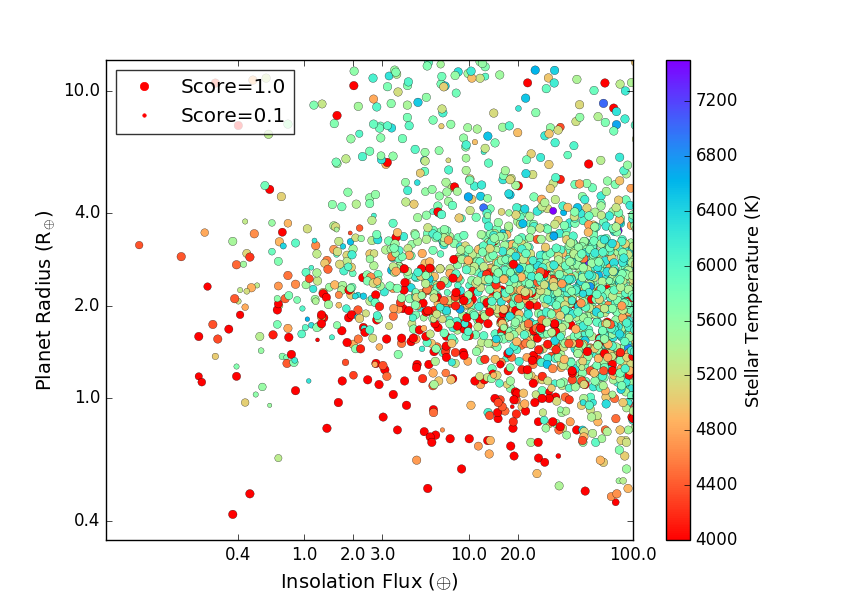
\includegraphics[width=1.1\linewidth]{fig-CatalogRadiusInsolScore.png}
    \caption{DR25 Exoplanet Candidates plotted as planet radius against Insolation Flux, in units of the flux that the Earth recieves from the Sun. The stellar temperature is given by the color of the circle and the size of the circle indicates the Disposition Score. The planet radii are derived from the MCMC fits. }
    \label{f:hzPlot}
\end{figure*}